% background chapter continued

\addtocontents{toc}{\protect\setcounter{tocdepth}{1}}

\section{Crawl Ordering Problem}\label{covfresh}
The purpose of a web crawler can be viewed as traversing the web graph. The crawling order appears naturally
to be breath-first problem (download pages following the links as they appear). But since the web is so
massive and still expanding such a crawling activity is considered infinite and the crawler itself can
be said to be \textit{random walker} with no purpose. Most of the commercial or even open source crawlers
have some sort of crawling order policy built into their system. It is a must for small-scale, special
purpose crawler to order the extracted URLs because the act of acquiring content is restricted by various
factors.
\begin{figure}[h!]
  \centering
  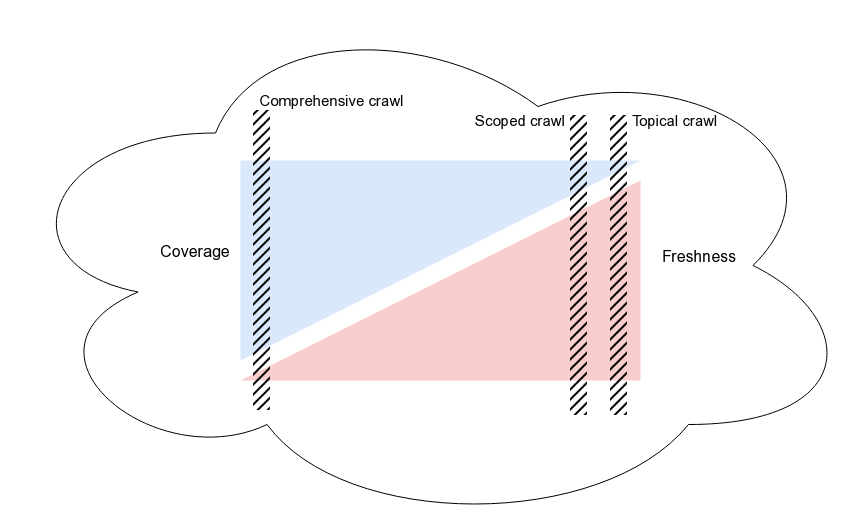
\includegraphics[width=15cm,height=12cm,keepaspectratio]{../media/crawler/crawl-ordering.png}
  \caption{Crawl ordering based on Coverage vs. Freshness}
  \label{fig:crawlorder}
\end{figure}

\noindent
\textbf{Coverage:} Focus is on fetching pages that the crawler deems required. 
\\
\textbf{Freshness:} Here the focus is on revisting, redownloading already visited pages. Since web 2.0,
pages are capable of dynamically changing content and popularity of Single Page Applications(SPA) has
enabled rendering data through view logic controlled by javascript.
\\
\\
As shown in the figure \ref{fig:crawlorder}, \textit{Comprehensive Crawling}\cite{trends} focuses on maximizing coverage by reaching out to content of all types.
A particular page $p$ is weighted important by counting external links outside current site's perimeter. Crawl order policies like Breath-first Search, PageRank, and other variations are applied. Such activity
is carried out by Commericial Search Engines.
\\
\\
On the other hand, \textit{Scoped Crawling}\cite{trends} narrows its
crawling activity to certain portion of the web i.e only crawl a specific category (e.g everything about Stock Market). The crawling order is determined based on a degree to which a page $p$ falls under its umbrella.
In constrast to Comprehensive, a Scoped crawler is suitable for data-mining tasks by performing
data collection on topics of interest.\textit{Topical Crawling}\cite{trends} is a form of Scoped Crawling in which page relevance is determined by - given a  page $p$ links to another page $p`$ and is in-scope(within bounds) either directly or through a series of subsequent links. There are 3 techniques to order URLs to crawl.

\begin{enumerate}
\item Fish Search (Binary classification). Here, the relevance is measured by treating links within visited
  page either relevant/irrelevant a certain height.
\item The relevance is estimated by doing textual analysis on text surrounding a link in a visited page $p$
  that points to yet-to-be visited page $q$.
\item Train and query a Machine Learning classifier to get the score of a set of topics of interest to crawl.
\end{enumerate}

\noindent
This crawler has to balance its greediness level by considering page relevance. It is possible that an already relevant page $p$ may not always yield a new relevant page but it might after going through
several links of irrelevant pages. If the crawler is designed to be too greedy then it will have zero
coverage which in turn means it won't discover new pages in its journey. A decay factor can be used to
allow irrelevant fetches with an ultimate intention of finding relevant page of interest.
\\
\\
Finally, freshness is the attribute that makes the design of crawler being either continuous or non-continuous. The question of balancing content coverage and freshness in a crawler is solely a decision of entity behind it. A \textit{batch crawling}\cite{trends} design requires restarting of a crawler at periodic interval to download revised content of previously crawled pages. A \textit{continuous} or \textit{incremental crawling}\cite{trends} design
would be technically a program that never terminates to revisit previously crawled pages.


\addtocontents{toc}{\protect\setcounter{tocdepth}{3}}